\documentclass{beamer}

\usepackage[utf8]{inputenc}
\input{../helper}

\title{Introdução à Computação \\ definindo funções em C}
\author{Alexandre Rademaker}
\date{}

\begin{document}

\begin{frame}
 \maketitle
\end{frame}


\begin{frame}[allowframebreaks,fragile]{funções}

  C e quase todas as linguagens modernas nos permitem escrever
  funções, às vezes também conhecidas como procedimentos, métodos ou
  sub-rotinas. Funções permitem: organização, reuso e simplificação.

  Modularização é importante para clareza e manutenção de código.

  Podemos pensar em uma função como uma \emph{caixa preta} que recebe
  zero ou mais entradas e produz uma saída.

  Ao \emph{usarmos} uma função, não precisamos saber detalhes de sua
  implementação.

  \framebreak

  O contrato de uma função é sua \emph{assinatura}. O comportamento
  normalmente é estimado com base no nome. A maioria das funções tem
  nomes óbvios e são bem documentadas.

  \begin{center}
    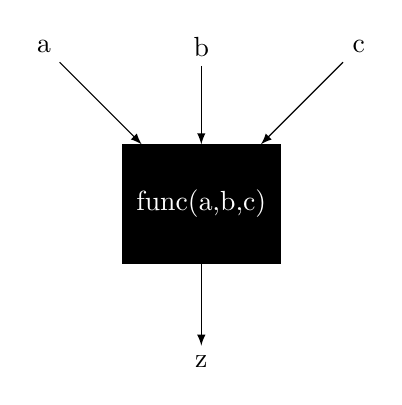
\begin{tikzpicture}[>=latex]
      % Draw the three numbers
      \node at (0,0) (num1) {a};
      \node at (2,0) (num2) {b};
      \node at (4,0) (num3) {c};
      
      % Draw the function box and arrow
      \node[draw, fill=black,text=white, minimum width=2cm, minimum height=1.5cm] at (2,-2) (func) {func(a,b,c)};
      \draw[->] (num1) -- (func);
      \draw[->] (num2) -- (func);
      \draw[->] (num3) -- (func);
      
      % Draw the output number and arrow
      \node at (2,-4) (output) {z};
      \draw[->] (func) -- (output);
    \end{tikzpicture}
  \end{center}

  \framebreak

  Funções podem ser declaradas antes da função \ilcode{main}

  {\texttt
    {\color{teal} return-type} {\color{red} name}({\color{blue} argument-list});}

  Exemplo:

  {\texttt
    {\color{teal} int} {\color{red} add\_two\_ints}({\color{blue} int\ a, int\ b});}

  Esta função recebe duas entradas, os nomes são para serem
  referenciadas internamente na função. Nada especial sobre estes
  nomes, podem ser simples.

  \framebreak

  Função podem ser definidas, seu comportamento especificado. Como os
  \emph{argumentos} devem ser usados para produzir a
  saída.\vspace{.5cm}

  \begin{lstlisting}[style=normalc]
    float mult_two_reals(float x, float y);
    
    float mult_two_reals(float x, float y)
    {
      float product = x * y;
      return product;
    }
  \end{lstlisting}

  \framebreak

  Agora, pense como podemos definir \ilcode{add_two_ints}?\vspace{.5cm}

  \begin{lstlisting}[style=normalc]
    int add_two_ints(int x, int y);
    
    int add_two_ints(int x, int y)
    {
      
    }
  \end{lstlisting}

  \framebreak

  Agora, pense como podemos definir \ilcode{add_two_ints}?\vspace{.5cm}

  \begin{lstlisting}[style=normalc]
    int add_two_ints(int x, int y)
    {
      int sum;
      sum = x + y;
      return sum;
    }
  \end{lstlisting}

  \framebreak

  Agora, pense como podemos definir \ilcode{add_two_ints}?\vspace{.5cm}

  \begin{lstlisting}[style=normalc]
    int add_two_ints(int x, int y)
    {
      int sum = x + y;
      return sum;
    }
  \end{lstlisting}

  \framebreak

  Agora, pense como podemos definir \ilcode{add_two_ints}?\vspace{.5cm}

  \begin{lstlisting}[style=normalc]
    int add_two_ints(int a, int b)
    {
      int sum = 0;
      if(a > 0)
        for(int i = 0; i < a; sum++, i++);
      else
        for(int i = a; i < 0; sum--, i++);
      if(b > 0)
        for(int i = 0; i < b; sum++, i++);
      else
        for(int i = b; i < 0; sum--, i++);
      return sum;
    }
  \end{lstlisting}

  \framebreak

  Para chamar uma função, passamos os \emph{argumentos} adequados e
  usamos o \emph{retorno} de forma apropriada (tipo adequado).

  Lembre-se que funções podem não receber argumentos, \ilcode{void}
  nos parâmetros.

  As vezes funções podem não retornar valor, declaramos que o retorno
  é \ilcode{void}.

\end{frame}

\begin{frame}[allowframebreaks,fragile]{exemplo}

  Declare uma função chamada \ilcode{valid_triangle} que usa três
  números reais que representam os comprimentos dos três lados de um
  triângulo como seus argumentos e retorna true ou false, dependendo
  se esses três comprimentos são capazes de formar um triângulo.

  Observe as seguintes fatos sobre triângulos:

  Um triângulo só pode ter lados com comprimento positivo.

  A soma dos comprimentos de quaisquer dois lados do triângulo deve
  ser maior que o comprimento do terceiro lado.

  \framebreak

  \begin{lstlisting}[style=normalc]
    bool valid_triangle(float x, float y, float z) {
      // all positive sides
      if (x <= 0 || y <= 0 || z <= 0) {
        return false;
      }
      // sum of any two sides greater than third
      if ((x + y <= z) || (x + z <= y) ||
          (y + z <= x)) {
        return false;
      }
      // we're good!
      return true;
    }
  \end{lstlisting}

\end{frame}


\begin{frame}[allowframebreaks,fragile]{níveis de abstração}

  \lstinputlisting[style=normalc,caption=src/meow2.c]{src/meow3.c}

  \framebreak

  Usando parâmetros podemos alterar o nível de abstração de nosso
  código.

  \lstinputlisting[style=normalc,caption=src/meow3.c]{src/meow4.c}

\end{frame}  


\begin{frame}[allowframebreaks,fragile]{parâmetros e argumentos}

  \begin{lstlisting}[style=normalc,caption=src/mario5.c]
    int get_size(void);
    void print_grid(int n);
    
    int main(int argc, string argv[]) {
      int x = get_size();
      print_grid(x);
    }
  \end{lstlisting}

  A variável \ilcode{x} foi declarada em \ilcode{main}. Seu valor foi
  passado como argumento e atribuído ao parâmetro \ilcode{n} da função
  \ilcode{print\_grid}.

  \framebreak

  Em programação, \emph{parâmetro} e \emph{argumento} são termos
  usados em conjunto para referir-se à passagem de valores para uma
  função ou método.

  Um \emph{parâmetro} é um valor definido na declaração da função,
  indicando o tipo e nome do valor esperado pela função.

  Um \emph{argumento} é o valor real passado para um parâmetro na chamada
  da função.
  
\end{frame}


\end{document}

%%% Local Variables:
%%% mode: latex
%%% TeX-master: t
%%% End:
